%%%%%%%%%%%%%%%%%%%%%%%%%%%%%%%%%%%%%%%%%%%%%%%%%%%%%%%%%%%%%%%
%
% Welcome to Overleaf --- just edit your LaTeX on the left,
% and we'll compile it for you on the right. If you open the
% 'Share' menu, you can invite other users to edit at the same
% time. See www.overleaf.com/learn for more info. Enjoy!
%
%%%%%%%%%%%%%%%%%%%%%%%%%%%%%%%%%%%%%%%%%%%%%%%%%%%%%%%%%%%%%%%
\documentclass{beamer}
%Information to be included in the title page:
\title{CMake and Toolchains: Introduction}
\subtitle{ESE PROG-5}
\usepackage{listings}
\usepackage{multicol}
\usepackage{dirtree}

\usepackage{minted}
\usepackage{tikz}
\usetikzlibrary{
    calc,
    shapes.misc,
    shapes.geometric,
    arrows, 
    arrows.meta, 
    fit, 
    positioning, 
    shapes.symbols, 
    chains, 
    mindmap,
    decorations.pathmorphing,
    decorations.markings,
    patterns,
    backgrounds,
    intersections,  
}
\usecolortheme{beaver}
\definecolor{backgroundColor}{HTML}{e50056}
\definecolor{bannerColor}{HTML}{1B262C}
\def\bannerOpacity{0.9}
\def\bannerWidth{0.8}
\def\bannerPadding{60pt}  
\def\bannerTopMargin{0cm}  

\tikzstyle {banner} = [
    below = \bannerTopMargin,
    fill=bannerColor,
    minimum width={\paperwidth},
    inner ysep = \bannerPadding,
    opacity = \bannerOpacity,
    text opacity = 1.0
]

\defbeamertemplate*{title page}{customized}[1][]
{
  \centering{
  \textcolor{white}{\usebeamerfont{title}\inserttitle}\par
  \bigskip
  \textcolor{white}{\usebeamerfont{subtitle}\insertsubtitle}\par
  \usebeamercolor[fg]{titlegraphic}\inserttitlegraphic
  }
}

\begin{document}
\begin{frame}


 \begin{tikzpicture}[
        overlay,
        background rectangle/.style={fill=backgroundColor}, 
        show background rectangle,
        remember picture
    ]
       % Add the logo in the bottom left
        \node[above right=10mm] at (current page.south west) {%
            
\includegraphics[width=0.25\linewidth]{figures/Han_logo_wit.png}};
    \end{tikzpicture}
\titlepage
\end{frame}

\begin{frame}[fragile]
\frametitle{How to compile a file..}
To explain how a normal toolchain works, we start with a normal source file:
hello\_world.c. \\ \bigskip
We want to compile and link this to an executable we can run natively on our pc: \\
\textbf{Linux/Mac:} \\
Using the GCC compiler:
\begin{lstlisting}[language=bash]
 $ GCC hello_world.c -o hello_world
 $ ./hello_world
\end{lstlisting} 

\textbf{Windows:} \\
Using the MSVC compiler:
\begin{lstlisting}[language=VBScript]
 > cl hello_world.c
 > hello_world 
\end{lstlisting}
\end{frame}

\begin{frame}
\frametitle{Toolchain process:}

\begin{multicols}{2}[]
The toolchain will execute the following steps: \\
1. Compile the source file to a object file (machine code).\\
2. Link the file with external compiled library files and the linker script (definition of the memory spaces).\\
3. When developing for embedded systems, utilities like Openocd or the Segger suite of tools might be used for debugging and programming.

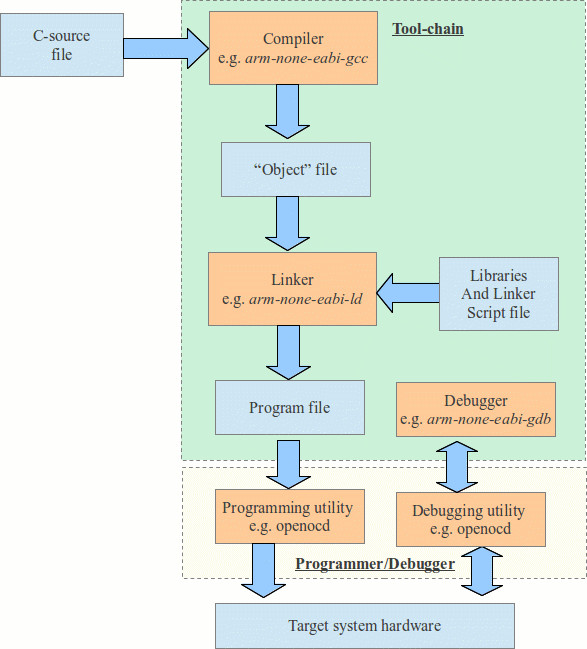
\includegraphics[width=\linewidth]{figures/toolchain_overview.jpg}
\end{multicols}
\end{frame}

\begin{frame}
\frametitle{Compiling to object files}
\scriptsize
The compiler does the following when compiling files in to object files: \\
1. \textbf{Preprocessing:} \\
- The compiler executes any directives specified in the source code (lines beginning with \#, such as \#include and \#define). \\
- It includes header files, expands macros, and performs other tasks to prepare the source code for compilation. \\\\
2. \textbf{Compilation:} \\
- The compiler translates the preprocessed C code into assembly code. \\
- It checks the syntax of the C code, ensuring it adheres to language standards, and reports any errors it encounters. \\\\
3. \textbf{Assembly:} \\
- The assembler converts the assembly code into machine code. \\
- The output is stored in an object file with a .o or .obj extension.\\\\
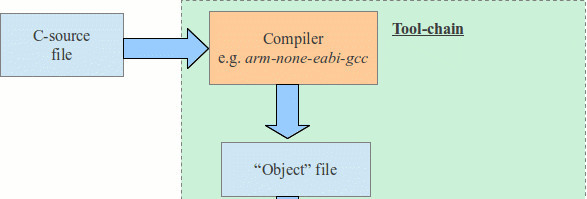
\includegraphics[scale = 0.25]{figures/toolchain_overview_compiling_step.jpg}
\end{frame}

\begin{frame}[fragile]
\frametitle{Demo: Looking at the preprocessor, compiler and assembler output}
GCC can be instructed to print the preprocessor output to the terminal using the -E parameter. To analyze the output we want to print it to a file using the "\textgreater" character.
\begin{lstlisting}[language=bash]
% gcc src/main.c lib/i2c.c lib/spi.c lib/uart.c 
-I lib/ -E > preprocessor_output
\end{lstlisting}
% \begin{block}{Question}
%     How many times does the file content of the stdio.h file get pasted in the preprocessor output?
% \end{block}
\end{frame}

\begin{frame}[fragile]
\begin{block}{Answer}
    3 Times! We have 3 source files utilizing the printf function. Each source file will be compiled separately and linked together. Meaning 3 copies of the printf are needed to make it compile.
\end{block}
\textbf{Let's now take a look at the object files... Again gcc can be instructed to only compile and not link the object files in a binary... What does the binary hide?}\\
We can do this using the gcc command with -C option (this forces compiler not to link):
\begin{lstlisting}[language=bash]
% gcc src/main.c lib/i2c.c lib/spi.c lib/uart.c -c
\end{lstlisting}
And then observing it with objdump..
\begin{block}{Question}
Without optimization flags and special compiler flags, how does the compiler handle constant strings inside the printf statement?
\end{block}
\end{frame}

\begin{frame}[fragile]
\tiny
\begin{block}{Remark: Memory sections}
When a program is compiled and linked, the resulting executable contains various pieces of information that are used both at load time and runtime, such as the program’s code, data, and additional metadata. Object files have a specific memory layout that organizes these different types of information into various sections. Understanding this memory layout is essential for debugging and optimizing compiled programs.\\
\textbf{Basic sections}
\begin{description}[leftmargin=!]
  \item[Text Segment (\texttt{.text}):] \ 
Contains the executable code (machine instructions) of the program. \\
Typically marked as read-only to prevent the program from accidentally modifying its own instructions.

 \item[Data Segment:] \ 
    Further divided into the Initialized (\texttt{.data}) and Uninitialized (\texttt{.bss}) Data segments.
    \begin{itemize}
       \item[] \texttt{.data}: Contains global and static variables that are initialized in the code. It holds the actual data values.
       \item[] \texttt{.bss}: Contains global and static variables that are not explicitly initialized in the code. This section is typically zero-initialized by the operating system at runtime.
    \end{itemize}

 \item[Read-Only Data Segment (\texttt{.rodata}):] \ 
Contains constants and string literals which should not be modified during the execution. \\
Marked as read-only.

\item[Heap:] \ 
    Memory segment used for dynamic memory allocation. \\
    Grows at runtime as more memory is dynamically allocated (e.g., with \texttt{malloc} in C).

\item[Stack:] \ 
    Contains function call frames, local variables, and control information for function calls. \\
    Used for managing function calls and returns.
\end{description}
\textbf{Additional sections}
\begin{description}[leftmargin=!]
    \item[Symbol Table (symtab):] \
     Contains information about functions and variables in the code.
        Used by the linker and debugger.
    \item[Debug Information:] \
     Contains source file names, line numbers, and other debug information.
         Used by debuggers to map machine instructions back to source code lines.
    \item[Relocation Table:] \
     Contains information used by the linker to adjust the program’s memory addresses.
\end{description}
\end{block}
\end{frame}

\begin{frame}[fragile]
    \frametitle{The linker}
    % \begin{block}{Question}
    % What type of linking is most commonly used on microcontrollers and why?
    % \end{block}
\end{frame}

\begin{frame}

\frametitle{How to compile multiple files?}
Imagine the following use-case: \\
We want to compile a library with one main source file and a library containing multiple source files and header files. \\ \bigskip
The target is a RPI pico W microcontroller, the compiler used is the GCC compiler.
\dirtree{%
.1 Project folder.
.2 lib.
.3 i2c.c.
.3 i2c.h.
.3 spi.c.
.3 spi.h.
.3 uart.c.
.3 uart.h.
.2 src.
.3 main.c.
}
\end{frame}

\begin{frame}[fragile]
To compile all these files we would need to enter the following command:
\begin{lstlisting}[language=bash]
$ gcc-arm-none-eabi main.c lib/i2c.c lib/spi.c 
lib/uart.c -I lib/ -mcpu=cortex-m0plus 
-mthumb -O main.hex
\end{lstlisting}
As you might have noticed the length of the command has increased noticeably.\\ \bigskip
This of course doesn't work out well when having more files or/and having to set target specific options like error-checking and warnings. \\ \bigskip
What if there would be a solution to this... \\ \bigskip

\includegraphics[scale=0.2]{figures/oh-boy-here-ili724.jpg}
\end{frame}


\begin{frame}[fragile]
\frametitle{Make}
\begin{multicols}{2}[]
    \footnotesize
    - Make is a build automation tool used to manage and automate the build process of a project.\\
    - It uses a Makefile to specify how a program should be compiled and linked.\\
    - Make is very popular in the (embedded) Linux community as it is provided by default in the package repository's, and used when consistency is required.
    

\includegraphics[width=\linewidth]{figures/makefile_syntax.jpg}
\end{multicols}
    % Makefiles and solution files are nothing but a recipe.. \\
    % - Whereas makefiles are used mostly in unix-like systems and solution files in windows.
\end{frame}

\begin{frame}[fragile]
\frametitle{How does Make work?}
Makefiles are nothing but a recipe.. \\
It always contains: \\
- \textbf{Target}:  The output file to be built. \\
- \textbf{Dependencies}: Files that the target depends on.\\
- \textbf{Recipe}: A series of commands to produce the target from the dependencies.\\
Example of a rule: \\
\begin{lstlisting}[language=make]
    target: dependencies
    recipe
\end{lstlisting}
A very important thing Make will do is check the time stamps of the target file and dependencies. If no file was changed then make will exit, else it will continue with the next step: \textbf{run the recipe commands}. \\
Make executes the recipe commands to create the required target.
\end{frame}

\begin{frame}[fragile]
\frametitle{Makefile example for use-case defined in previous slide}
\tiny
\begin{lstlisting}[language=make]
# Compiler and Linker
CC = arm-none-eabi-gcc
LD = arm-none-eabi-ld
# Flags
CFLAGS = -mcpu=cortex-m0plus -mthumb

# Include paths, assuming the Pico SDK is installed and PICO_SDK_PATH is set
INCLUDE = -I$(PICO_SDK_PATH)/include

# Source files
LIB_SOURCES = lib/i2c.c lib/spi.c lib/uart.c
MAIN_SOURCE = src/main.c

# Object files
OBJS = $(LIB_SOURCES:.c=.o) $(MAIN_SOURCE:.c=.o)

# Output executable
OUTPUT = main.elf

# Default target
all: $(OUTPUT)

# Rule to compile source files to object files
%.o: %.c
	$(CC) $(CFLAGS) $(INCLUDE) -c $< -o $@

# Rule to link object files and create executable
$(OUTPUT): $(OBJS)
	$(LD) $(LDFLAGS) $(OBJS) -o $(OUTPUT)

# Clean target
clean:
	rm -f $(OBJS) $(OUTPUT)
\end{lstlisting}
\end{frame}

\begin{frame}
\frametitle{When to use Make and what are the limitations}
\textbf{When to use:} \\
- Simple to moderately sized projects \\
- When you need full control over the build-process \\
- Projects primarily targeting or using the Unix or GNU+Linux operating system \\
\textbf{Limitations:} \\
- Makefiles are platform and compiler specific. \\
Meaning you have to write different Makefiles for different platforms, or include complex conditional logic in a single Makefile.
\end{frame}

\begin{frame}
\frametitle{Microsoft Visual Studio solution files}
A solution file for c/c++ projects most of the time have a .vcxproj file extension.\\
A solution files is composed of a XML file describing the build targets, compiler settings and build environment specifics. \\ \bigskip
Solution files are only used under Windows and can't be used natively under any other operating system. \\ \bigskip
Due to the XML format, visual studio solution files are pretty easy to understand, however they don't give you the absolute control a Makefile would give you.
\end{frame}

\begin{frame}[fragile]
\tiny
\frametitle{Solution file example}
\begin{lstlisting}[language=xml]
    <?xml version="1.0" encoding="utf-8"?>
<Project DefaultTargets="Build" ToolsVersion="15.0" xmlns="http://schemas.microsoft.com/developer/msbuild/2003">

  <!-- Global Properties -->
  <PropertyGroup Label="Globals">
    <ProjectGuid>{CE8885D6-7C94-40B7-8F0A-0C5ED9CFA1F5}</ProjectGuid>
    <Keyword>Win32Proj</Keyword>
    <!-- Other Global Properties -->
  </PropertyGroup>

  <!-- Configuration Properties -->
  <PropertyGroup Condition="'$(Configuration)|$(Platform)'=='Debug|Win32'" Label="Configuration">
    <ConfigurationType>Application</ConfigurationType>
    <!-- Other Configuration Properties -->
  </PropertyGroup>

  <!-- Import Default Settings -->
  <Import Project="$(VCTargetsPath)\Microsoft.Cpp.Default.props" />

  <!-- Other Settings and Configurations -->

  <!-- List of Files to Compile -->
  <ItemGroup>
    <ClCompile Include="main.cpp" />
    <!-- Other Source Files -->
  </ItemGroup>

  <!-- Import Targets -->
  <Import Project="$(VCTargetsPath)\Microsoft.Cpp.targets" />
</Project>
\end{lstlisting}
\end{frame}

\begin{frame}
    \frametitle{When to solution files and what are the limitations}
    \footnotesize
    \textbf{When to use:}\\
    - \textbf{When everyone is working with visual studio.} \\
    Some advanced features like IntelliSense, GUI-based configuration and some of the debug tools are only available when using solution files in visual studio. \\
    - \textbf{When developing for Windows.} \\
    For software targeting Windows platforms, .vcxproj files provide easier setup and integration with Windows-specific libraries and frameworks.\\
    - \textbf{When working with Mixed Languages.} \\
    Visual Studio supports multiple languages (C++, C\#, F\#, etc.) in a single solution, making it easier to work with mixed-language projects.\\
    \textbf{Limitations:}\\
    - \textbf{Very Windows bound..}\\
    Solution files are closely tied to the Microsoft ecosystem. \\ They are not as platform-agnostic as some other build systems.\\
    - \textbf{Complexity} \\
    Although XML is very human readable, it will become very unreadable quickly when having to build big projects (lots of files) with a lot of project-specific settings. \\
    - \textbf{Less Fine-grained Control} \\
    .vcxproj files may not offer as much fine-grained control over the build process as some other systems, like make.
\end{frame}

\begin{frame}
\frametitle{Ninja build files}
What if I told you there is another tool, yes another one... Introducing Ninja...\\
Ninja is a small build system that is designed to be fast. It focuses on improving the speed of incremental builds, where only a subset of the source files are modified. It was originally designed to speed up the builds for Google Chrome and is used in the Android operating system's build system as well.\\ \bigskip

\textbf{How Ninja works}  \\
- Ninja uses a simple text file (build.ninja) as a build file. \\
- This file contains rules and dependencies for building the project. \\
- Unlike other build systems, build.ninja files are not written by hand. Instead, they are typically generated by a higher-level build system like CMake or Meson. \\
\end{frame}

\begin{frame}[fragile]
\frametitle{Build.ninja example}
\tiny
\begin{lstlisting}
# The Ninja build file for compiling the hello project.

# Variables.
cc = gcc
cflags = -Wall -O2
lflags = -o

# Rule to compile C files.
rule cc
  command = $cc $cflags -c $in -o $out

# Rule to link object files into an executable.
rule link
  command = $cc $lflags $out $in

# Build edges.
build main.o: cc main.c
build hello.o: cc hello.c

# Link the object files into the final executable.
build hello: link main.o hello.o

\end{lstlisting}
\end{frame}

\begin{frame}
\frametitle{When to use Ninja and what are the limitations}
\footnotesize
\textbf{When to use:}\\
- \textbf{Large codebases}\\
For extremely large codebases, Ninja can significantly reduce the build time, especially for incremental builds, as it focuses on improving the speed of such builds.\\
- \textbf{Cross-Platform Development} \\
Ninja is platform-agnostic, making it a good choice for projects that need to be built on multiple operating systems. \\
- \textbf{Complex dependencies} \\
 Ninja effectively manages complex dependencies in a project, ensuring that only the necessary parts of the project are rebuilt, which helps in saving build time.\\
\textbf{Limitations}\\
- \textbf{Limited Functionality} \\
Ninja has fewer features compared to other build systems like CMake or Make. It’s generally used as a backend to these systems and doesn’t handle configuration or project setup.\\
- \textbf{Less Ideal for Small Projects} \\
For smaller projects, the overhead of setting up Ninja (or another system to generate Ninja build files) might not be justified, and simpler build tools might be more appropriate.
\end{frame}


\begin{frame}
\frametitle{Recap: }
\footnotesize
   Each build system has its own strengths and weaknesses. \\
   When we recap on previous slides we can conclude the following: \\ \bigskip
    Use make when:\\
        You want cross-platform compatibility and fine-grained control over the build process, suitable for smaller to medium projects.\\ \bigskip

    Use .vcxproj when:\\
        Working primarily on Windows, using the Visual Studio IDE, and dealing with multi-language projects.\\ \bigskip

    Use Ninja when: \\  
        Working with large codebases where fast build times are crucial, especially when using build systems like CMake or Meson that can generate Ninja build files. \\ \bigskip

Ultimately, the best choice depends on your specific project requirements, including the size and complexity of your project, your target platform, and your preferred development tools and environment.
\end{frame}

\begin{frame}[fragile]
\frametitle{How do I decide?}
\begin{columns}
\column{0.5\textwidth}
Good question!\\
The answer is... *drumroll* \\It depends! \\ \bigskip
If requirements are not too strict on the toolchain, there are tools that make this decision *cough* *cough* easier.\\ \bigskip
Easier in the sense that the tool makes the decision for you. \\
Take eclipse CDT or CMake \\
\column{0.5\textwidth}

\includegraphics[scale=0.145]{figures/it-depends.jpg}
\end{columns}
\end{frame}

\begin{frame}
\frametitle{CMake: Introduction}
Ah yes finally. Let's skip over eclipse anyway, as it is not a worthy contender anyway...\\ \bigskip
\textbf{But what is CMake?}\\
CMake is a tool which \textbf{generates build files}. It mostly used in conjunction with native build environments such as Make, Apple's Xcode, and Microsoft Visual Studio. \\
\begin{columns}
    \column{0.6\textwidth}
    CMake uses it's own scripting language (CMakeLists.txt files) to define build settings, targets, and dependencies.\\ \bigskip
    Although CMake is very well documented, it still might require some getting used to (just like any language :p).\\
    \column{0.4\textwidth}
    
\includegraphics[width=0.9\textwidth]{figures/dive into cmake.jpg}
\end{columns}
\end{frame}

\begin{frame}[fragile]
\frametitle{CMake: example CMakeLists.txt}
CMake has both separate build scripts for libraries and the main project source files. \\
\begin{columns}
    \column{0.5\linewidth}
    Project CMakeLists.txt
    \column{0.5\linewidth}
    Library CMakeLists.txt
\end{columns}
\tiny
\begin{columns}
    \column{0.5\linewidth}
    
   \begin{minted}{cmake}
# Set the minimum required version of CMake
cmake_minimum_required(VERSION 3.10)

# Set the project name
project(Hello_world)

# Add the executable
add_executable(Hello_world src/main.c)

# Link the executable with the library
target_link_libraries(Hello_world PeripheralDriver)
        
    \end{minted}
    
    \column{0.5\linewidth}
   
   \begin{minted}{cmake}
# Add library source files
add_library(PeripheralDriver STATIC lib/i2c.c 
                                    lib/spi.c 
                                    lib/uart.c)
                                            
# Add current folder "lib/" as include directory
target_include_directories(PeripheralDriver "." )
 \end{minted}
\end{columns}
\end{frame}

\begin{frame}[fragile]
\frametitle{CMake: Syntax deep dive}
\begin{itemize}
    \item \textbf{Comments:} \\
        Start with a \# symbol. \\
        \begin{minted}{cmake}
# This is a comment
        \end{minted}
    \item \textbf{Variables:} \\
         Variables are case-sensitive and can be set with the set() command. \\
         \begin{minted}{cmake} 
set(MY_VARIABLE "Hello, World!")
         \end{minted}
    \item \textbf{Commands:} \\
        Commands are case-insensitive and called using parentheses ().\\
        \begin{minted}{cmake}
# Outputs a message during the cmake generation step
message("This is a message") 
        \end{minted}
\end{itemize}
\end{frame}

\begin{frame}[fragile]
    \begin{itemize}
        \item \textbf{Control Structures:} \\
        CMake supports control structures such as if, while, and foreach.
        \begin{minted}{cmake}
if(MY_VARIABLE STREQUAL "Hello, World!")
    message("Variable is Hello, World!")
endif()
        \end{minted}
        \item \textbf{Project Information:} \\
        Set the project name and version. Can only be set once in a project, is mostly set right after setting the minimum cmake version.
        \begin{minted}{cmake}
project(MyProject VERSION 1.0)
        \end{minted}
        \item \textbf{Include directories:} \\
        Sets include directory of the executable target.
        \begin{minted}{cmake}
include_directories(${CMAKE_SOURCE_DIR}/include)
        \end{minted}
    \end{itemize}
\end{frame}

\begin{frame}[fragile]
    \begin{itemize}
        \item \textbf{Add Executable:} \\
        Define an executable target and its source files.
        \begin{minted}{cmake}
add_executable(MyExecutable main.cpp util.cpp)
        \end{minted}
        \item \textbf{Add Library:} \\
        Define a library target and its source files.
        \begin{minted}{cmake}
add_library(MyLibrary STATIC lib1.cpp lib2.cpp)
        \end{minted}
        \item \textbf{Target Link Libraries:} \\
        Link libraries to targets.
        \begin{minted}{cmake}
target_link_libraries(MyExecutable MyLibrary)
        \end{minted}
        \item \textbf{Custom Commands and Targets:} \\
        Define custom build commands and targets.
        \begin{minted}{cmake}
add_custom_command(...)
add_custom_target(...)
        \end{minted}
    \end{itemize}
\end{frame}

\begin{frame}[fragile]
\frametitle{CMake: Advanced commands and features}
CMake is a scripting language, that means it can also download dependencies like external libraries from GitHub. \\
\tiny
\begin{minted}{cmake}
# Include the ExternalProject module
include(ExternalProject)

# Set the minimum required version of CMake
cmake_minimum_required(VERSION 3.11) # ExternalProject_Add() requires at least CMake 3.11

# Set the project name
project(MyProject)

# Add the external project
ExternalProject_Add(
    name_of_the_external_project              # Name for the external project
    PREFIX ${CMAKE_BINARY_DIR}/_deps          # Download location
    GIT_REPOSITORY https://github.com/user/repo.git  # URL of the GitHub repo
    GIT_TAG main                              # Git branch, commit or tag to checkout
    CMAKE_ARGS -DCMAKE_INSTALL_PREFIX=<INSTALL_DIR>  # Installation directory
)

# You can then link against or add dependencies as needed
add_dependencies(your_target name_of_the_external_project)
\end{minted}
\end{frame}
\end{document}